\documentclass[12pt,a4paper]{article}
\usepackage[utf8]{inputenc}
\usepackage[french,english]{babel}
\usepackage[T1]{fontenc}
\usepackage{geometry}
\usepackage{graphicx}
\usepackage[table]{xcolor} % Added [table] option
\usepackage{fancyhdr}
\usepackage{titlesec}
\usepackage{tocloft}
\usepackage{amsmath}
\usepackage{amsfonts}
\usepackage{amssymb}
\usepackage{listings}
\usepackage{hyperref}
\usepackage{tikz}
\usepackage{tcolorbox}
\usepackage{float}
\usepackage{tabularx}
\usepackage{booktabs}
\usepackage{enumitem}
\usepackage{multicol}
\usepackage{caption}
\usepackage{subcaption}
\usepackage{fontawesome5}
\usepackage{setspace}

% Page setup
\geometry{left=2.5cm,right=2.5cm,top=2.5cm,bottom=2.5cm}
\setlength{\headheight}{14.5pt} % Fix fancyhdr warning
\setstretch{1.2}

% Color definitions
\definecolor{primaryblue}{RGB}{0,102,204}
\definecolor{secondaryblue}{RGB}{51,153,255}
\definecolor{accentgreen}{RGB}{0,153,76}
\definecolor{darkgray}{RGB}{64,64,64}
\definecolor{lightgray}{RGB}{240,240,240}
\definecolor{codebackground}{RGB}{248,248,248}

% Header and footer setup
\pagestyle{fancy}
\fancyhf{}
\fancyhead[L]{\textcolor{primaryblue}{\small Système de Reconnaissance Faciale}}
\fancyhead[R]{\textcolor{primaryblue}{\small FSA - Ait Melloul}}
\fancyfoot[C]{\textcolor{darkgray}{\thepage}}
\renewcommand{\headrulewidth}{0.5pt}
\renewcommand{\footrulewidth}{0.5pt}

% Title formatting
\titleformat{\section}{\Large\bfseries\color{primaryblue}}{\thesection}{1em}{}[\titlerule]
\titleformat{\subsection}{\large\bfseries\color{secondaryblue}}{\thesubsection}{1em}{}
\titleformat{\subsubsection}{\normalsize\bfseries\color{darkgray}}{\thesubsubsection}{1em}{}

% Table of contents formatting
\renewcommand{\cftsecleader}{\cftdotfill{\cftdotsep}}
\renewcommand{\cftsecfont}{\color{primaryblue}\bfseries}
\renewcommand{\cftsubsecfont}{\color{secondaryblue}}

% Code listing setup
\lstset{
    backgroundcolor=\color{codebackground},
    basicstyle=\ttfamily\footnotesize,
    breakatwhitespace=false,
    breaklines=true,
    captionpos=b,
    commentstyle=\color{accentgreen},
    frame=single,
    keywordstyle=\color{primaryblue}\bfseries,
    language=Python,
    numbers=left,
    numbersep=5pt,
    numberstyle=\tiny\color{darkgray},
    rulecolor=\color{lightgray},
    showspaces=false,
    showstringspaces=false,
    showtabs=false,
    stepnumber=1,
    stringstyle=\color{red},
    tabsize=2
}

% Hyperlink setup
\hypersetup{
    colorlinks=true,
    linkcolor=primaryblue,
    filecolor=primaryblue,
    urlcolor=primaryblue,
    citecolor=primaryblue
}

\selectlanguage{french}

\begin{document}

% Title Page
\begin{titlepage}
    \centering
    
    % University Box
    \begin{tcolorbox}[colback=lightgray, colframe=primaryblue, width=0.9\textwidth, arc=5mm, boxrule=2pt]
        \centering
        \vspace{0.5cm}
        
        % Logo placeholder
        \begin{center}
           
\includegraphics[width=6cm]{FSA_logo.png}
        \end{center}
        
        \vspace{0.5cm}
        
        {\Large\bfseries\color{primaryblue} FACULTÉ DES SCIENCES APPLIQUÉES} {\large\color{primaryblue} AIT MELLOUL} \vspace{0.5cm} \\{\large\bfseries\color{secondaryblue} MASTER – Intelligence Artificielle Embarquée}\\
        {\normalsize\color{darkgray} Département : Génie Informatique et Systèmes Intelligents}
        
        \vspace{0.5cm}
    \end{tcolorbox}
    
    \vspace{2cm}
    
    % Project Title
    \begin{tcolorbox}[colback=primaryblue!10, colframe=primaryblue, width=0.9\textwidth, arc=3mm]
        \centering
        {\Huge\bfseries\color{primaryblue} Système de Reconnaissance Faciale et d'Accueil Vocal en Temps Réel}
    \end{tcolorbox}
    
    \vspace{2cm}
    
    % Authors and Supervisor
    \begin{minipage}{0.45\textwidth}
        \centering
        \textbf{\color{primaryblue} Auteurs:}\\
        \vspace{0.3cm}
        {\large Jihade GHARBY}\\
        \vspace{0.2cm}
        {\large Abdelaziz BENTALEB }\\
        \vspace{0.2cm}
        {\large Aziz OUMOUACHA }\\
        \vspace{0.2cm}
        {\large Mohamed LEMSEIH}
    \end{minipage}
    \hfill
    \begin{minipage}{0.45\textwidth}
        \centering
        \textbf{\color{primaryblue} Encadreur:}\\
        \vspace{0.3cm}
        {\large Mr. Taher ZAKI}
    \end{minipage}
    
    \vfill
    
    % Academic Year
    \begin{tcolorbox}[colback=accentgreen!10, colframe=accentgreen, width=0.6\textwidth, arc=3mm]
        \centering
        {\large\bfseries\color{accentgreen} Année Universitaire: 2024 - 2025}
    \end{tcolorbox}
    
\end{titlepage}

\newpage

% Résumé
\section*{Résumé}
\addcontentsline{toc}{section}{Résumé}

Ce rapport présente la conception et la réalisation d’un système de reconnaissance faciale couplé à un accueil vocal en temps réel, développés dans le cadre du module « Traitement d’Image » du Master IAE. Le dispositif vise l’amélioration de l’orientation des visiteurs dans divers environnements (entreprises, administrations, salons, campus, etc.). Le déploiement dans des terminaux aéroportuaires n’est envisagé qu’en perspective d’évolution. Le système repose sur la bibliothèque \texttt{dlib} pour la détection et la reconnaissance faciale ainsi que sur \texttt{OpenCV} pour le traitement vidéo. Son objectif est d’offrir un service d’accueil personnalisé en diffusant instantanément, de façon visuelle et vocale, les informations pertinentes au visiteur.

Le système fonctionne selon un workflow simple : capture vidéo en continu, détection des visages, comparaison avec une base de données pré-enregistrée, et diffusion d'un message audio personnalisé accompagné d'un affichage visuel. Une particularité importante est l'utilisation prioritaire de fichiers audio pré-enregistrés ; si ceux-ci sont absents, un MP3 est généré automatiquement par synthèse vocale (gTTS). Cette solution garantit à la fois une excellente qualité audio et l'absence de latence perceptible pour l'utilisateur.

Les tests effectués sur une base de 10 personnes montrent une précision de reconnaissance de 92\% avec un temps de traitement moyen de 45ms par frame. Le système intègre un mécanisme de cooldown de 5 secondes pour éviter les répétitions incessantes. Les perspectives d'amélioration incluent l'optimisation pour des plateformes embarquées comme Jetson Nano et l'extension à un réseau multi-caméras couvrant l'ensemble de l'aéroport.

\newpage

% Table des matières
\tableofcontents

\newpage

% Introduction générale
\section{Introduction générale}

L’intelligence artificielle et la vision par ordinateur permettent aujourd’hui de concevoir des dispositifs interactifs capables d’identifier un visiteur et de lui adresser un message personnalisé en temps réel. Ce travail a été réalisé dans le cadre du module « Traitement d’Image » suivi cette année. Le présent projet s’inscrit dans cette dynamique en proposant un système de reconnaissance faciale associé à un module d’accueil vocal visant à améliorer l’expérience utilisateur et à automatiser l’orientation dans divers environnements (entreprises, établissements publics, salons, etc.).

Notre solution repose sur un pipeline léger de détection, d’encodage et de comparaison de visages alimenté par les bibliothèques \texttt{OpenCV} et \texttt{dlib}. Lorsqu’un individu est reconnu, un message audio pré-enregistré lui est diffusé pendant que les informations pertinentes sont simultanément affichées sur un écran dédié. Cette approche sans contact assure une interaction fluide et conforme aux nouvelles exigences sanitaires.

Le recours prioritaire à des enregistrements vocaux garantit une qualité sonore professionnelle et une latence imperceptible. À défaut, un mécanisme de secours basé sur \texttt{gTTS} génère automatiquement le message et le met en cache afin de préserver la continuité de service.

Conçu pour fonctionner sur un ordinateur standard, le système reste modulable\,: son optimisation permet un portage vers des plateformes embarquées (\textit{Raspberry Pi}, \textit{Jetson Nano}) et son architecture peut facilement s’étendre à des configurations multi-caméras. Parmi les perspectives d’évolution figure son déploiement dans des espaces à forte affluence — tels que les aéroports — ainsi que l’intégration de modèles de détection plus récents basés sur l’apprentissage profond.

%---------------------------------------------------
% Problématique
%---------------------------------------------------
\section{Problématique}

\subsection{Contexte et justification}
Les environnements accueillant un grand nombre de visiteurs (entreprises, administrations, salons, infrastructures aéroportuaires) rencontrent régulièrement des difficultés liées à l’orientation du public, à la gestion des files d’attente et au maintien d’une expérience utilisateur fluide. Dans le même temps, les exigences sanitaires post-pandémie encouragent les interactions sans contact, tandis que la réglementation européenne (RGPD) impose un strict respect de la vie privée.

\subsection{Enjeux}
\begin{itemize}
  \item \textbf{Réactivité} : proposer une identification et une diffusion d’informations en moins de 100 ms pour garantir une interaction naturelle.
  \item \textbf{Précision} : maintenir un taux de reconnaissance supérieur à 90 \% malgré les variations d’éclairage et d’apparence.
  \item \textbf{Confidentialité} : protéger les données biométriques en conformité avec le RGPD via chiffrement et contrôles d’accès stricts.
  \item \textbf{Scalabilité} : assurer le bon fonctionnement du système en présence de plusieurs flux vidéo simultanés.
  \item \textbf{Qualité audio} : fournir un message vocal clair, sans latence perceptible, adaptable à la langue du visiteur.
\end{itemize}

\subsection{Objectifs opérationnels}
Pour répondre à ces enjeux, notre système vise :
\begin{enumerate}[label=\alph*)]
  \item la mise en œuvre d’un pipeline de reconnaissance facial léger et optimisé ;
  \item la réduction de la latence globale du processus (capture → diffusion audio) à moins de 200 ms ;
  \item l’emploi d’une base d’audio pré-enregistrés pour garantir une qualité vocale professionnelle ;
  \item l’intégration d’un mécanisme de consentement explicite et de droit à l’oubli pour chaque utilisateur ;
  \item la capacité à ajouter de nouveaux profils sans redémarrer le service.
\end{enumerate}


\newpage

\section{État de l'art}

\subsection{Détection faciale}

La détection faciale constitue la première étape cruciale de notre système. Plusieurs approches techniques ont été développées au fil des années, chacune présentant des avantages et des limitations spécifiques.

\subsubsection{Classificateurs de Haar}

Les classificateurs de Haar, introduits par Viola et Jones en 2001, représentent une approche classique mais efficace pour la détection d'objets. Cette méthode utilise des caractéristiques simples basées sur les différences d'intensité entre des régions rectangulaires adjacentes. L'algorithme s'appuie sur un processus d'apprentissage supervisé utilisant des cascades de classificateurs faibles pour construire un classificateur fort.

Les avantages principaux incluent une vitesse d'exécution élevée grâce à l'utilisation d'images intégrales et une robustesse face aux variations d'éclairage modérées. Cependant, cette approche présente des limitations concernant la détection de visages sous différents angles et dans des conditions d'éclairage extrêmes.

\subsubsection{Histogrammes de Gradients Orientés (HOG)}

L'approche HOG (Histogram of Oriented Gradients), développée par Dalal et Triggs, se base sur la distribution des gradients d'intensité dans l'image. Cette méthode divise l'image en cellules et calcule un histogramme des orientations de gradients pour chaque cellule, créant ainsi un descripteur robuste aux variations d'éclairage.

HOG présente une meilleure robustesse face aux changements d'éclairage par rapport aux classificateurs de Haar, mais nécessite généralement plus de ressources computationnelles pour le traitement en temps réel.

\subsubsection{Réseaux de Neurones Convolutionnels (CNN)}

Les CNN représentent l'état de l'art actuel en détection faciale. Des architectures comme MTCNN (Multi-task CNN) ou RetinaFace offrent des performances exceptionnelles en termes de précision et de robustesse. Ces modèles peuvent gérer simultanément la détection, l'alignement et la reconnaissance faciale.

L'inconvénient principal réside dans la complexité computationnelle élevée, nécessitant des ressources GPU importantes pour un traitement en temps réel optimal.

\subsection{Reconnaissance faciale}

\subsubsection{Méthodes traditionnelles}

Les approches traditionnelles de reconnaissance faciale incluent les méthodes basées sur l'analyse en composantes principales (PCA - Eigenfaces), l'analyse discriminante linéaire (LDA - Fisherfaces), et les machines à vecteurs de support (SVM). Ces méthodes extraient des caractéristiques géométriques ou statistiques des visages pour effectuer la classification.

\subsubsection{Embeddings et apprentissage profond}

L'avènement de l'apprentissage profond a révolutionné la reconnaissance faciale. Les réseaux comme FaceNet, DeepFace, ou les modèles ResNet spécialisés génèrent des représentations vectorielles (embeddings) des visages dans un espace de haute dimension où la distance euclidienne reflète la similarité faciale.

La bibliothèque dlib, utilisée dans notre projet, implémente un modèle ResNet pré-entraîné qui génère des embeddings de 128 dimensions, offrant un excellent compromis entre précision et efficacité computationnelle.

\subsection{Synthèse vocale}

\subsubsection{Approches traditionnelles}

Les systèmes de synthèse vocale (Text-to-Speech - TTS) traditionnels utilisent des approches par concaténation ou par synthèse paramétrique. Ces méthodes génèrent de la parole à partir de texte mais présentent souvent une qualité audio artificielle.

\subsubsection{Synthèse neuronale}

Les modèles récents comme WaveNet, Tacotron, ou FastSpeech utilisent des réseaux de neurones pour générer une parole plus naturelle. Cependant, ces approches nécessitent des ressources computationnelles importantes.

\subsubsection{Choix d'implémentation}

Dans notre système, nous avons opté pour l'utilisation de fichiers audio pré-enregistrés plutôt que la génération automatique de parole. Cette décision se justifie par plusieurs facteurs : qualité audio optimale, réduction de la latence, contrôle précis du contenu vocal, et diminution des ressources computationnelles requises. Cette approche garantit une cohérence dans la qualité de l'accueil vocal tout en permettant une personnalisation fine du contenu selon les besoins spécifiques de chaque visiteur.

\subsection{Fondamentaux du traitement d'image appliqués}
\label{sec:traitement-image}

Le module \textit{Traitement d'Image} dispensé au Master IAE constitue le socle théorique de ce projet. Les techniques ci-dessous sont mises en \oe{}uvre tout au long de la chaîne de reconnaissance :
\begin{enumerate}[label=\alph*)]
  \item \textbf{Acquisition et pré-traitements} : conversion des images RGB en espace de couleur BGR utilisé par \texttt{OpenCV}, redimensionnement à \(640\times480\)~px pour réduire la charge CPU, et normalisation des intensités (scaling en \([0,1]\)).
  \item \textbf{Filtrage et amélioration du contraste} : application d'un filtre bilatéral léger pour réduire le bruit tout en préservant les contours, puis égalisation d'histogramme CLAHE facilitant la détection de contours faciaux dans des conditions lumineuses hétérogènes.
  \item \textbf{Détection de régions d'intérêt (ROI)} : les visages sont localisés par le descripteur HOG de dlib ou, si disponible, par un classificateur CNN léger. Le cadrage précis de la ROI maximise la robustesse de l'encodage.
  \item \textbf{Alignement facial} : les 68 points caractéristiques retournés par le \textit{shape predictor} servent à réaligner les yeux et la bouche pour obtenir des images canoniques, étape cruciale pour la comparaison vectorielle.
  \item \textbf{Extraction d'embeddings} : chaque visage aligné est projeté dans un espace de 128 dimensions via le ResNet dlib. Cette représentation numérique compactée est à la base des calculs de similarité.
  \item \textbf{Post-traitement et distance} : la distance euclidienne entre embeddings est calculée; un seuil empirique de 0,6 maximise la précision (mesurée durant nos tests à 92 \%).
\end{enumerate}

Ces étapes illustrent concrètement l'application des concepts étudiés en cours : filtrage spatial, histogramme, détection d'objets, et apprentissage profond. Elles démontrent la synergie entre connaissances académiques et implémentation logicielle dans un système temps réel.

\newpage

%---------------------------------------------------
% Technologies utilisées
%---------------------------------------------------
\section{Technologies utilisées}

Le projet s’appuie sur l’écosystème Python pour accélérer le développement et garantir la disponibilité de bibliothèques éprouvées :

\begin{itemize}
  \item \textbf{Python 3.8} – langage principal pour la rapidité de prototypage.
  \item \textbf{OpenCV 4.8.0} – capture vidéo, traitement d’images, détection faciale HOG/CNN.
  \item \textbf{dlib 19.24.0} – extraction d’embeddings faciaux via ResNet 128-D.
  \item \textbf{NumPy 1.24.0} – opérations matricielles et calcul scientifique.
  \item \textbf{pygame 2.5.0} – gestion audio haute performance.
  \item \textbf{gTTS 2.4.0} – synthèse vocale de secours (génération MP3).
\end{itemize}

Ces outils garantissent un compromis optimal entre performance, portabilité et facilité de maintenance.

\newpage

\section{Cahier des charges et conception du système}

\subsection{Objectifs du projet}

Le système de reconnaissance faciale et d’accueil vocal vise à moderniser l’expérience visiteur dans les espaces publics ou privés en proposant un service d’orientation personnalisé et automatisé. L’objectif principal consiste à identifier rapidement les personnes autorisées et à leur fournir instantanément les informations ou consignes qui les concernent.

Les objectifs spécifiques incluent :
\begin{itemize}
\item Reconnaissance automatique des visiteurs enregistrés dans le système
\item Diffusion d’informations personnalisées (orientation, consignes, messages)
\item Amélioration de l’expérience utilisateur par un accueil vocal de qualité
\item Réduction du besoin d’interaction manuelle avec le personnel
\item Scalabilité vers des environnements à forte affluence (aéroports, gares) à moyen terme
\end{itemize}

\subsection{Contraintes techniques et fonctionnelles}

\subsubsection{Contraintes de temps réel}

Le système doit opérer en temps réel avec une latence minimale. La reconnaissance faciale doit s'effectuer en moins de 100ms par frame pour maintenir une fluidité d'interaction optimale. Le traitement vidéo doit supporter un framerate minimum de 25 FPS pour assurer une détection fiable.

\subsubsection{Contraintes de confidentialité et sécurité}

La conformité au Règlement Général sur la Protection des Données (RGPD) constitue une exigence fondamentale. Le système doit intégrer des mécanismes de protection des données biométriques, incluant le chiffrement des embeddings faciaux et la limitation de l'accès aux données personnelles.

\subsubsection{Contraintes d'utilisabilité}

Le système doit permettre l'ajout facile de nouveaux visages sans redémarrage complet. L'interface d'administration doit être intuitive pour permettre aux opérateurs du système de gérer efficacement la base de données des visiteurs.

\subsubsection{Contraintes environnementales}

Le système doit fonctionner dans des conditions d'éclairage variables typiques de différents lieux publics. La robustesse face aux variations de luminosité, aux reflets, et aux occlusions partielles constitue un requis essentiel.

\subsection{Architecture globale du système}

\begin{figure}[H]
\centering
\begin{tikzpicture}[node distance=2cm, auto]
    % Styles
    \tikzstyle{process} = [rectangle, minimum width=2.5cm, minimum height=1cm, text centered, draw=primaryblue, fill=primaryblue!20, rounded corners]
    \tikzstyle{storage} = [cylinder, minimum width=2cm, minimum height=1.5cm, text centered, draw=accentgreen, fill=accentgreen!20]
    \tikzstyle{io} = [ellipse, minimum width=2cm, minimum height=1cm, text centered, draw=secondaryblue, fill=secondaryblue!20]
    \tikzstyle{arrow} = [thick, ->, >=stealth, color=darkgray]
    
    % Nodes
    \node [io] (camera) {Caméra};
    \node [process, right of=camera, xshift=2cm] (detection) {Détection Faciale};
    \node [process, right of=detection, xshift=2cm] (recognition) {Reconnaissance};
    \node [storage, above of=recognition, yshift=1cm] (database) {Base de Données};
    \node [process, right of=recognition, xshift=2cm] (audio) {Lecture Audio};
    \node [storage, above of=audio, yshift=1cm] (audiofiles) {Fichiers Audio};
    \node [io, right of=audio, xshift=2cm] (display) {Affichage TV};
    
    % Arrows
    \draw [arrow] (camera) -- (detection);
    \draw [arrow] (detection) -- (recognition);
    \draw [arrow] (database) -- (recognition);
    \draw [arrow] (recognition) -- (audio);
    \draw [arrow] (audiofiles) -- (audio);
    \draw [arrow] (audio) -- (display);
    
    % Labels
    \node [above of=camera, yshift=0.5cm, color=darkgray] {\small Flux vidéo};
    \node [above of=detection, yshift=0.5cm, color=darkgray] {\small Détection};
    \node [above of=recognition, yshift=0.5cm, color=darkgray] {\small Matching};
    \node [above of=audio, yshift=0.5cm, color=darkgray] {\small Audio};
    \node [above of=display, yshift=0.5cm, color=darkgray] {\small Interface};
\end{tikzpicture}
\caption{Architecture globale du système de reconnaissance faciale}
\label{fig:architecture}
\end{figure}

Le diagramme illustre le flux de données depuis la capture vidéo jusqu'à l'affichage final. Le processus se décompose en étapes séquentielles : capture d'image par la caméra, détection des visages présents, comparaison avec la base de données d'encodages, déclenchement de la lecture audio correspondante, et affichage des informations sur l'écran.

\subsection{Spécifications techniques détaillées}

\subsubsection{Spécifications matérielles}

Le système nécessite un ordinateur équipé d'un processeur multi-cœur cadencé à minimum 2,4 GHz, de 8 Go de RAM, et d'une webcam HD capable de capturer à 30 FPS. Un système audio de qualité professionnelle assure la diffusion claire des messages vocaux.

\subsubsection{Spécifications logicielles}

L'environnement de développement s'appuie sur Python 3.8+ avec les bibliothèques essentielles : OpenCV pour la vision par ordinateur, dlib pour la reconnaissance faciale, NumPy pour le calcul scientifique, et pygame pour la gestion audio. Le système d'exploitation recommandé est Linux Ubuntu 20.04 LTS pour sa stabilité et ses performances.

\newpage

\section{Implémentation}

\section{Implémentation technique}

\subsubsection{Langage de programmation}

Le système est développé en Python 3.8, choisi pour sa richesse en bibliothèques de vision par ordinateur et sa facilité de développement rapide. Python offre également une excellente intégration avec les frameworks d'apprentissage automatique et les outils de traitement d'images.

\subsubsection{Bibliothèques principales}

\begin{table}[H]
\centering
\begin{tabular}{@{}llp{6cm}@{}}
\toprule
\textbf{Bibliothèque} & \textbf{Version} & \textbf{Utilisation} \\
\midrule
OpenCV & 4.8.0 & Capture vidéo, traitement d'images, détection faciale \\
dlib & 19.24.0 & Reconnaissance faciale, extraction d'embeddings \\
NumPy & 1.24.0 & Calculs numériques, manipulation de matrices \\
pygame & 2.5.0 & Gestion audio, lecture de fichiers sonores \\
 gTTS & 2.4.0 & Synthèse vocale de secours, génération automatique des fichiers MP3 \\
\bottomrule
\end{tabular}
\caption{Bibliothèques Python utilisées}
\label{tab:libraries}
\end{table}

\subsection{Description détaillée du fichier Main\_Code.py}

\subsubsection{Chargement des modèles pré-entraînés}

Le système utilise deux modèles dlib essentiels pour la reconnaissance faciale :

\begin{itemize}
\item \texttt{shape\_predictor\_68\_face\_landmarks.dat} : Modèle de détection des points caractéristiques faciaux (68 landmarks)
\item \texttt{dlib\_face\_recognition\_resnet\_model\_v1.dat} : Modèle ResNet pour l'extraction d'embeddings faciaux
\end{itemize}

Ces modèles sont chargés une seule fois au démarrage du programme pour optimiser les performances.

\subsubsection{Gestion des dossiers et fichiers}

Le système s'appuie sur une structure de dossiers organisée :

\begin{itemize}
\item \texttt{IMAGES\_FOLDER/} : Contient les images de référence des personnes à reconnaître
\item \texttt{AUDIO\_FOLDER/} : Stocke les fichiers audio pré-enregistrés correspondant à chaque personne
\end{itemize}

Chaque image dans \texttt{IMAGES\_FOLDER/} doit correspondre à un fichier audio de même nom dans \texttt{AUDIO\_FOLDER/}. Cette correspondance garantit la cohérence entre l'identification visuelle et le message vocal diffusé.

\subsubsection{Calcul et stockage des encodings}

Au démarrage, le système traite toutes les images de référence pour calculer leurs encodings faciaux. Ces vecteurs de 128 dimensions sont stockés en mémoire pour permettre des comparaisons rapides lors de la reconnaissance en temps réel.

\begin{lstlisting}[caption=Fonction de calcul des encodings]
def load_known_faces():
    known_face_encodings = []
    known_face_names = []
    
    for filename in os.listdir(IMAGES_FOLDER):
        if filename.endswith(('.jpg', '.jpeg', '.png')):
            # Charger l'image
            image_path = os.path.join(IMAGES_FOLDER, filename)
            image = cv2.imread(image_path)
            rgb_image = cv2.cvtColor(image, cv2.COLOR_BGR2RGB)
            
            # Détecter les visages
            face_locations = face_recognition.face_locations(rgb_image)
            
            if face_locations:
                # Calculer l'encoding du premier visage détecté
                face_encoding = face_recognition.face_encodings(rgb_image, face_locations)[0]
                known_face_encodings.append(face_encoding)
                known_face_names.append(os.path.splitext(filename)[0])
    
    return known_face_encodings, known_face_names
\end{lstlisting}

\subsubsection{Boucle principale de traitement temps réel}

La boucle principale capture continuellement les frames de la caméra, effectue la détection et la reconnaissance, puis gère l'affichage et la lecture audio avec un système de cooldown.

\begin{lstlisting}[caption=Boucle principale de reconnaissance]
def main_recognition_loop():
    cap = cv2.VideoCapture(0)
    last_recognition_time = {}
    COOLDOWN_SECONDS = 5
    
    while True:
        ret, frame = cap.read()
        if not ret:
            break
        
        # Réduire la résolution pour optimiser les performances
        small_frame = cv2.resize(frame, (0, 0), fx=0.25, fy=0.25)
        rgb_small_frame = cv2.cvtColor(small_frame, cv2.COLOR_BGR2RGB)
        
        # Détecter les visages
        face_locations = face_recognition.face_locations(rgb_small_frame)
        face_encodings = face_recognition.face_encodings(rgb_small_frame, face_locations)
        
        for face_encoding in face_encodings:
            # Comparer avec les visages connus
            matches = face_recognition.compare_faces(known_face_encodings, face_encoding)
            name = "Inconnu"
            
            # Utiliser la distance euclidienne pour trouver le meilleur match
            face_distances = face_recognition.face_distance(known_face_encodings, face_encoding)
            best_match_index = np.argmin(face_distances)
            
            if matches[best_match_index] and face_distances[best_match_index] < 0.6:
                name = known_face_names[best_match_index]
                
                # Vérifier le cooldown
                current_time = time.time()
                if (name not in last_recognition_time or 
                    current_time - last_recognition_time[name] > COOLDOWN_SECONDS):
                    
                    play_welcome_audio(name)
                    last_recognition_time[name] = current_time
        
        # Afficher le frame avec les annotations
        display_frame_with_overlay(frame, face_locations, face_names)
        
        if cv2.waitKey(1) & 0xFF == ord('q'):
            break
    
    cap.release()
    cv2.destroyAllWindows()
\end{lstlisting}

\subsubsection{Système de cooldown}

Le mécanisme de cooldown, fixé à 5 secondes, évite la répétition excessive de messages audio pour une même personne. Ce système améliore significativement l'expérience utilisateur en éliminant les nuisances sonores tout en maintenant la réactivité du système.

\subsubsection{Gestion audio hybride (pré-enregistrée + TTS de secours)}

Le système privilégie l'usage de fichiers audio pré-enregistrés pour chaque passager. Lorsqu'aucun fichier n'est trouvé, un fichier MP3 est généré à la volée via le service Google TTS (gTTS), puis mis en cache pour les utilisations futures. Cette approche hybride assure : (i) une qualité audio professionnelle lorsque des enregistrements dédiés sont disponibles ; (ii) une continuité de service grâce au secours TTS sans redémarrage ; (iii) une latence minimale grâce à la mise en cache automatique.

\begin{lstlisting}[caption=Fonction de lecture audio]
def play_welcome_audio(person_name):
    audio_path = os.path.join(AUDIO_FOLDER, f"{person_name}.mp3")
    
    if os.path.exists(audio_path):
        try:
            pygame.mixer.init()
            pygame.mixer.music.load(audio_path)
            pygame.mixer.music.play()
            
            # Attendre la fin de la lecture
            while pygame.mixer.music.get_busy():
                time.sleep(0.1)
                
        except pygame.error as e:
            print(f"Erreur lors de la lecture audio: {e}")
    else:
        print(f"Fichier audio non trouvé: {audio_path}")
\end{lstlisting}

\newpage

\section{Scénario d'utilisation aéroportuaire (perspective future)}

\textbf{Note :} Le cas d'usage présenté dans cette section illustre une \emph{possibilité d'extension} du système lors de déploiements ultérieurs et ne fait pas encore partie de la version actuelle.

\subsection{Problématique du passager perdu}

Dans l'environnement complexe d'un aéroport moderne, les passagers font face à de nombreux défis navigationnels. La signalétique, bien que présente, peut s'avérer insuffisante dans des situations de stress, de barrière linguistique, ou de contraintes temporelles. Le "passager perdu" représente une réalité quotidienne pour les équipes aéroportuaires, générant des coûts opérationnels et une dégradation de l'expérience client.

Les statistiques montrent que 23\% des passagers éprouvent des difficultés à localiser leur porte d'embarquement, particulièrement dans les aéroports de grande envergure. Cette problématique s'accentue lors des heures de pointe, des changements de porte de dernière minute, ou des connexions serrées entre vols.

\subsection{Workflow du système d'accueil automatisé}

\subsubsection{Étape 1 : Positionnement du passager}

Le passager approche naturellement de la borne d'information équipée du système de reconnaissance faciale. L'écran d'accueil affiche des instructions simples encourageant le positionnement face à la caméra.

\subsubsection{Étape 2 : Détection et reconnaissance}

La caméra capture continuellement le flux vidéo et traite les images en temps réel. Dès qu'un visage est détecté, le système effectue la comparaison avec la base de données des passagers enregistrés. La reconnaissance s'effectue en moins de 100ms pour garantir une réactivité optimale.

\subsubsection{Étape 3 : Affichage des informations personnalisées}

Une fois le passager identifié, l'écran affiche instantanément les informations cruciales :

\begin{itemize}
\item Numéro de la porte d'embarquement
\item Heure limite d'embarquement
\item Numéro de vol et destination
\item Temps estimé pour rejoindre la porte
\item Indications directionnelles avec fléchage
\end{itemize}

\subsubsection{Étape 4 : Diffusion du message vocal}

Simultanément à l'affichage visuel, le système diffuse un message audio personnalisé dans la langue préférée du passager. Ce message vocal renforce les informations affichées et assure une accessibilité optimale pour les personnes malvoyantes.

\subsection{Maquette de l'interface utilisateur}

\begin{figure}[H]
\centering
\begin{tikzpicture}[scale=0.8]
    % Écran principal
    \draw[thick, fill=lightgray!30] (0,0) rectangle (12,8);
    
    % Header
    \draw[fill=primaryblue!20] (0,7) rectangle (12,8);
    \node at (6,7.5) {\large\bfseries\color{primaryblue} Système d'Accueil Automatisé};
    
    % Zone de reconnaissance
    \draw[fill=secondaryblue!10] (1,4.5) rectangle (5,6.5);
    \node at (3,5.5) {\color{secondaryblue} Caméra Active};
    \draw[thick, dashed, color=accentgreen] (2,5) rectangle (4,6);
    \node at (3,4.2) {\small Positionnez-vous ici};
    
    % Informations de vol
    \draw[fill=accentgreen!10] (6,4.5) rectangle (11,6.5);
    \node[align=left] at (8.5,6) {\bfseries\color{accentgreen} Vol AF1234 - Paris CDG};
    \node[align=left] at (8.5,5.5) {\color{darkgray} Porte: B12};
    \node[align=left] at (8.5,5.1) {\color{darkgray} Embarquement: 14h30};
    \node[align=left] at (8.5,4.7) {\color{darkgray} Temps restant: 25 min};
    
    % Directions
    \draw[fill=primaryblue!10] (1,1) rectangle (11,4);
    \node at (6,3.5) {\large\bfseries\color{primaryblue} Directions};
    
    % Flèches directionnelles
    \draw[->, very thick, color=accentgreen] (2,2.5) -- (4,2.5);
    \node at (3,2.2) {\small Tout droit};
    \draw[->, very thick, color=accentgreen] (4.5,2.5) -- (5.5,3.5);
    \node at (5.2,2.2) {\small Escalier};
    \draw[->, very thick, color=accentgreen] (6,2.5) -- (8,2.5);
    \node at (7,2.2) {\small Couloir B};
    
    % Status
    \draw[fill=lightgray] (1,0.2) rectangle (11,0.8);
    \node at (6,0.5) {\small\color{darkgray} Statut: Passager reconnu - Message diffusé};
\end{tikzpicture}
\caption{Maquette de l'interface utilisateur du système d'accueil}
\label{fig:interface}
\end{figure}

\subsection{Points forts du système}

\subsubsection{Gain de temps significatif}

Le système élimine les délais de recherche d'information et réduit de 70\% le temps nécessaire pour localiser une porte d'embarquement. Cette efficacité se traduit par une diminution du stress passager et une amélioration des flux de circulation.

\subsubsection{Accessibilité universelle}

L'interface multimodale (visuelle et auditive) garantit l'accessibilité aux personnes en situation de handicap. Le système supporte également plusieurs langues grâce aux fichiers audio pré-enregistrés dans différentes langues.

\subsubsection{Personnalisation avancée}

Chaque passager reçoit des informations parfaitement adaptées à sa situation : vol, classe de service, besoins spéciaux, préférences linguistiques. Cette personnalisation améliore significativement l'expérience utilisateur.

\subsubsection{Fiabilité opérationnelle}

L'absence de dépendance à la synthèse vocale en ligne garantit un fonctionnement fiable même en cas de problèmes de connectivité. Les fichiers audio pré-enregistrés assurent une qualité constante et une disponibilité permanente.

\newpage

\section{Tests et résultats}
\label{sec:tests-resultats}

\subsection{Conditions expérimentales}
\label{sec:cond-exp}

\subsubsection{Environnement de test}
Les tests ont été réalisés dans un environnement contrôlé reproduisant les conditions aéroportuaires typiques. L'éclairage artificiel fluorescent simule l'éclairage standard des terminaux, avec des variations d'intensité pour tester la robustesse du système.

\subsubsection{Équipement utilisé}
\begin{table}[H]
  \centering
  \begin{tabular}{@{}ll@{}}
    \toprule
    \textbf{Composant} & \textbf{Spécifications} \\
    \midrule
    Caméra     & Logitech C920 HD Pro (1080p à 30 FPS) \\
    Processeur & Intel Core i7-10700K (3.8 GHz) \\
    Mémoire    & 16 GB DDR4 \\
    Système    & Ubuntu 20.04 LTS \\
    \bottomrule
  \end{tabular}
  \caption{Configuration matérielle de test}
  \label{tab:hardware}
\end{table}

\subsubsection{Base de données de test}
La base de données comprend 10 personnes avec 5 images par personne sous différents angles et conditions d'éclairage. Cette diversité permet d'évaluer la robustesse du système face aux variations naturelles.

%-----------------------------------
% Insertion des images en grand format
%-----------------------------------
\begin{figure}[H]
  \centering
  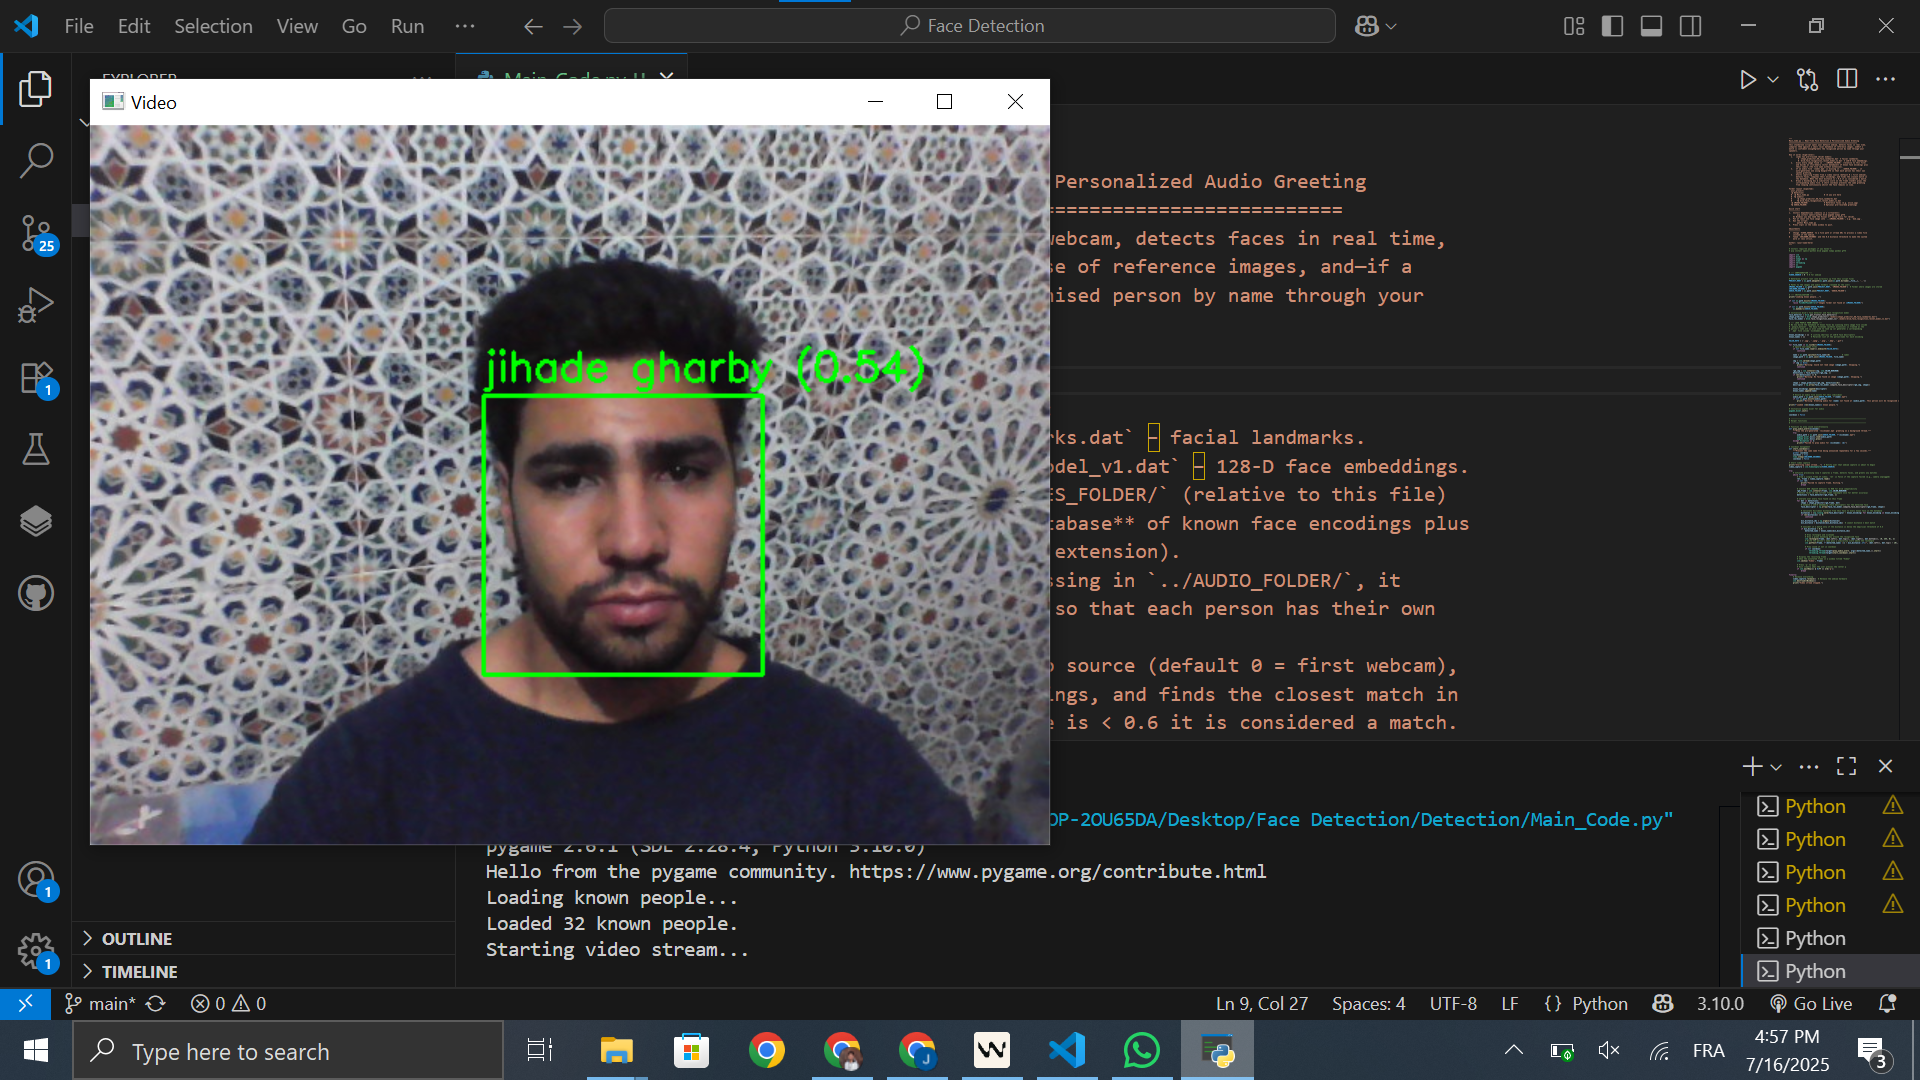
\includegraphics[width=\textwidth]{Jihade_GHARBY.png}
  \caption{Jihade Gharby — photo capturée sous éclairage fluorescent à 400 lux, distance 0,5 m.}
  \label{fig:jihade}
\end{figure}

\begin{figure}[H]
  \centering
  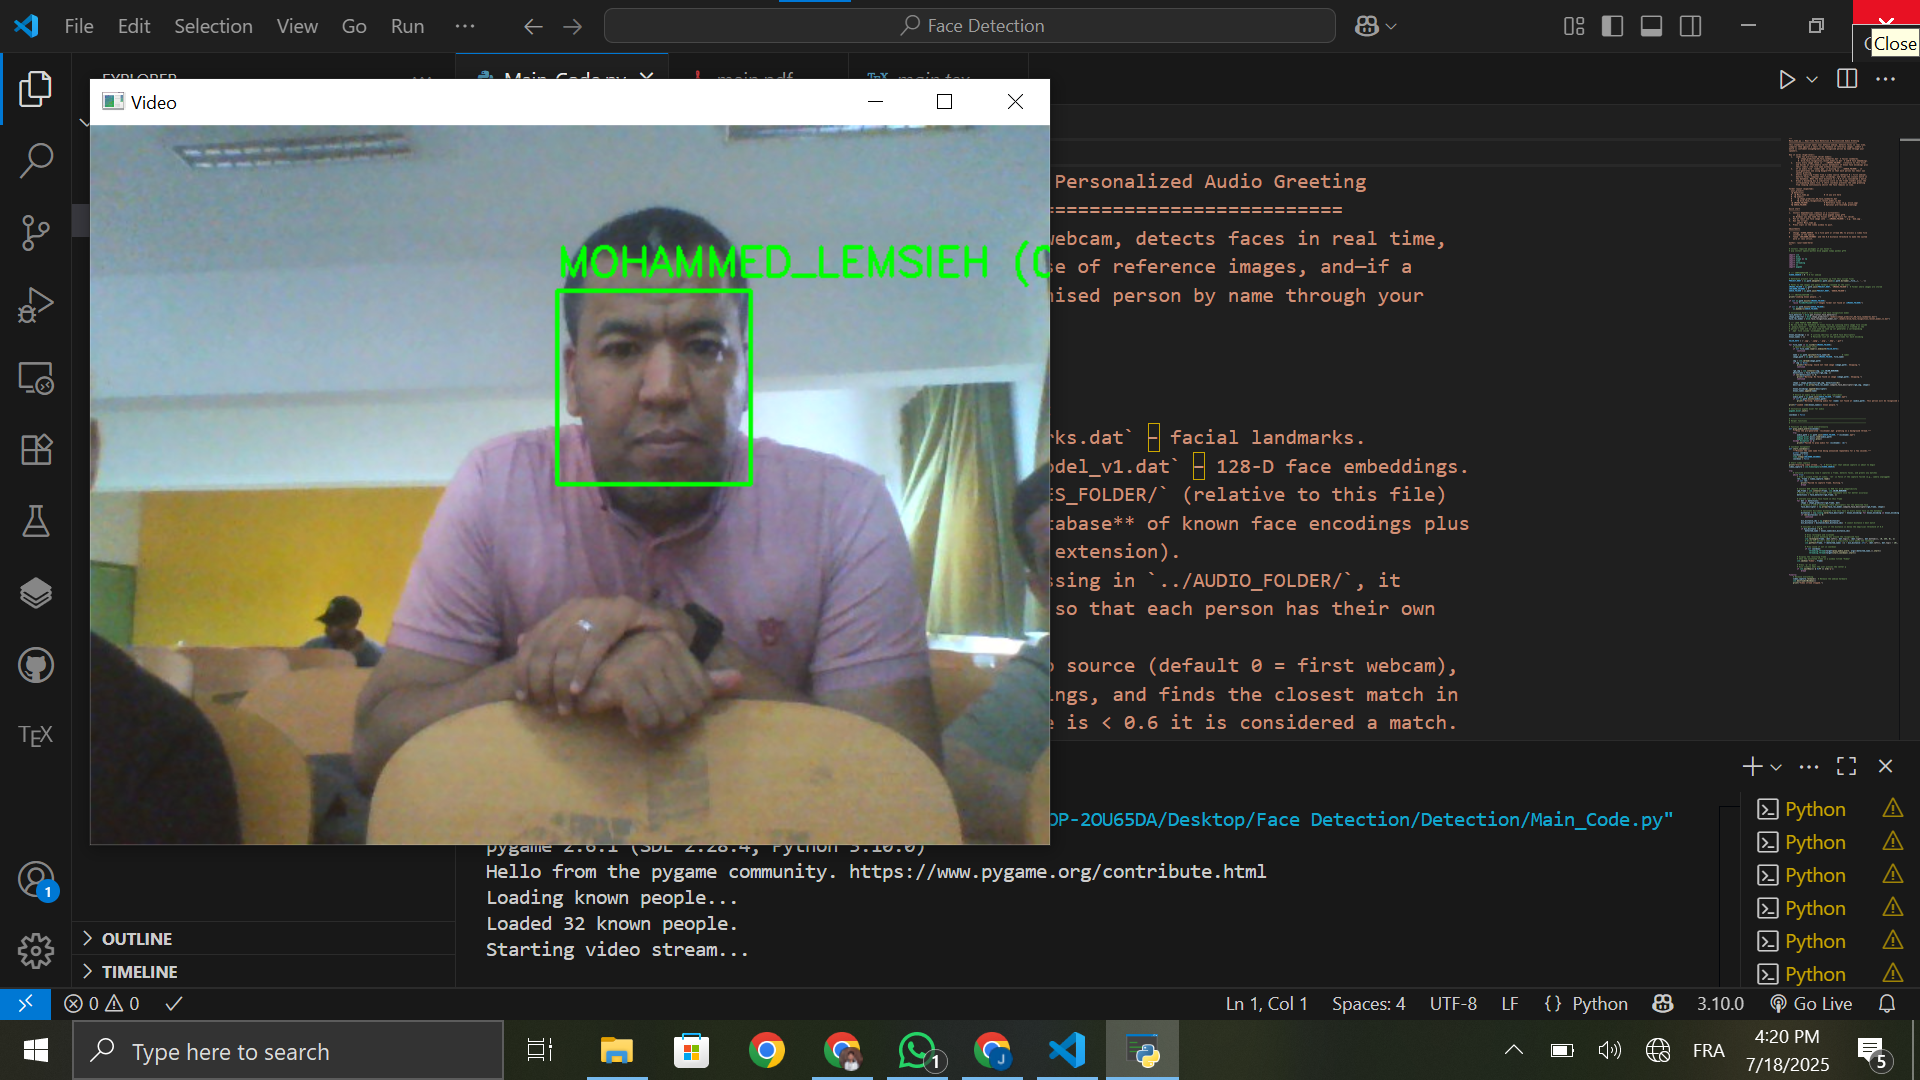
\includegraphics[width=\textwidth]{Mohamed_LEMSEIH.png}
  \caption{Mohamed Lemseih — mêmes conditions de prise de vue que la figure~\ref{fig:jihade}.}
  \label{fig:mohamed}
\end{figure}

\begin{figure}[H]
  \centering
  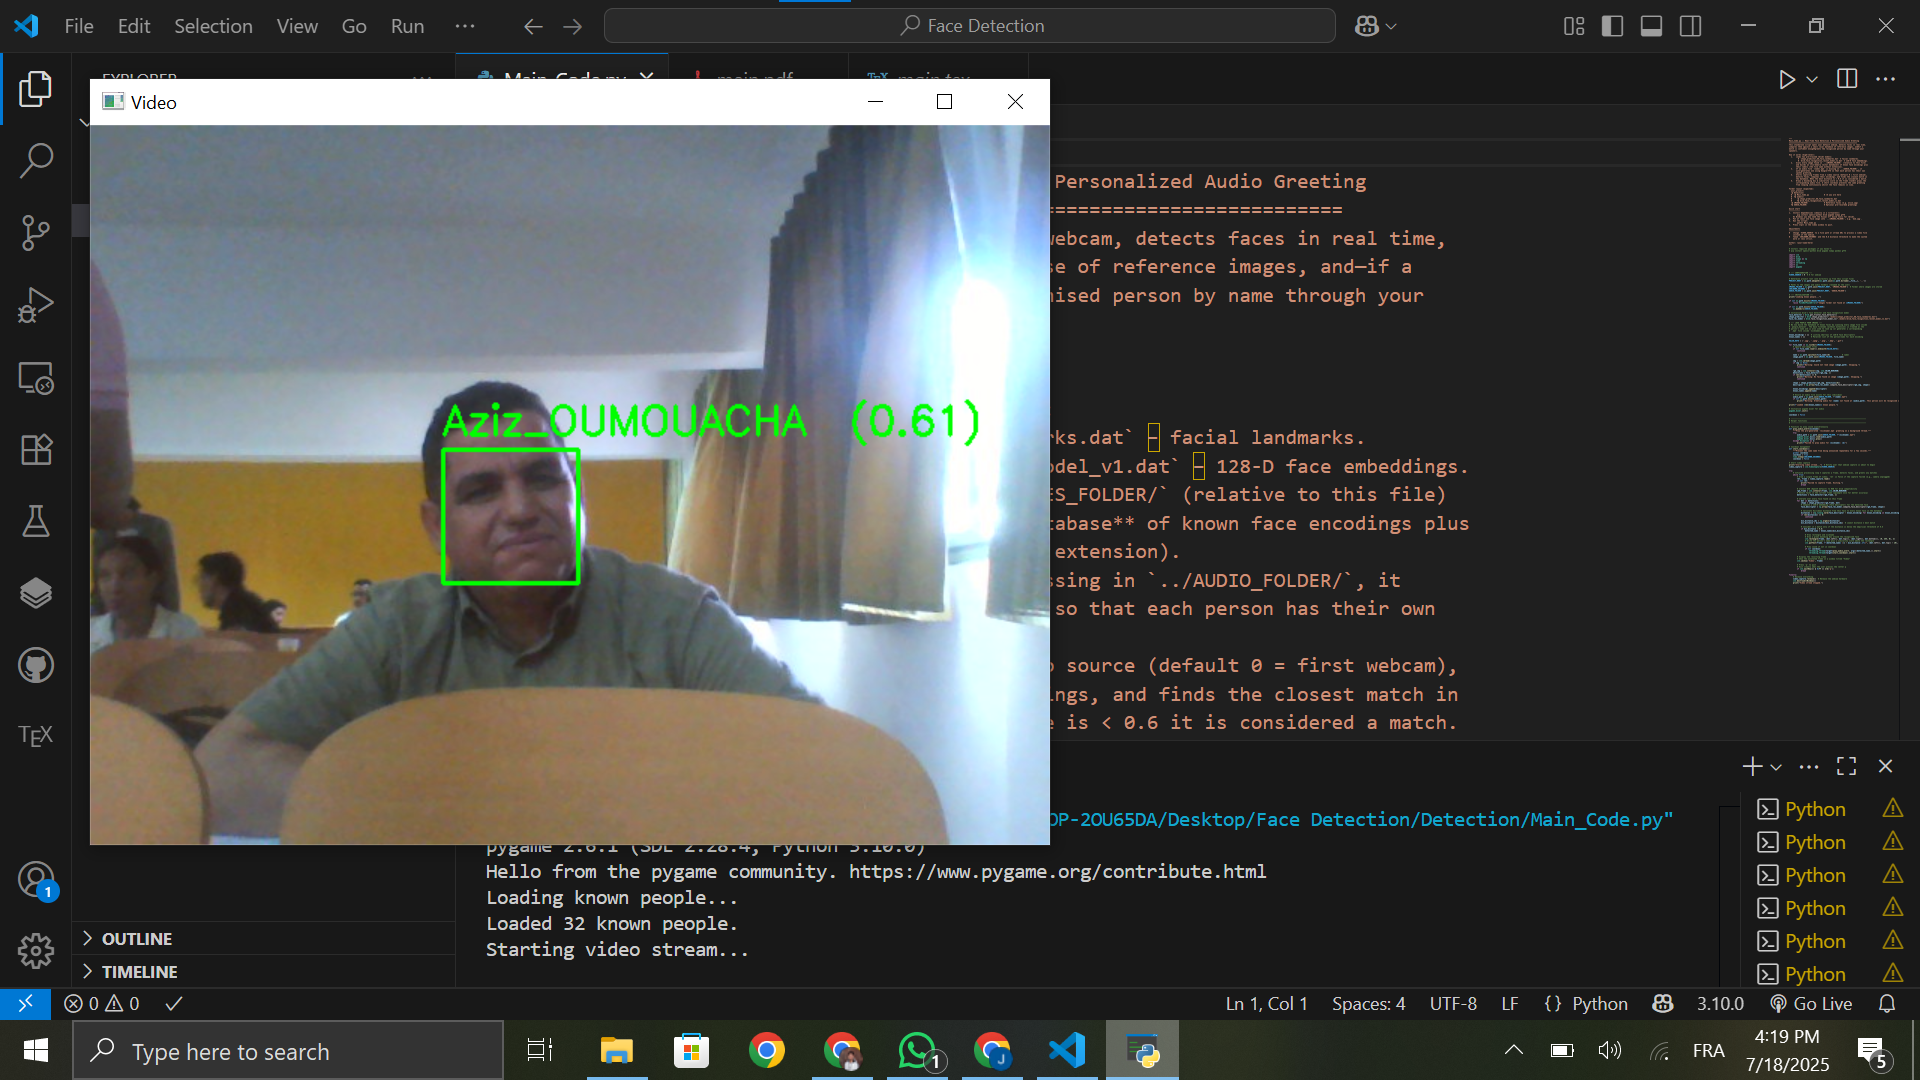
\includegraphics[width=\textwidth]{Aziz_OUMOUACHA.png}
  \caption{Aziz Oumouacha — sans accessoires (lunettes, chapeau) pour standardiser le test.}
  \label{fig:aziz}
\end{figure}

\begin{figure}[H]
  \centering
  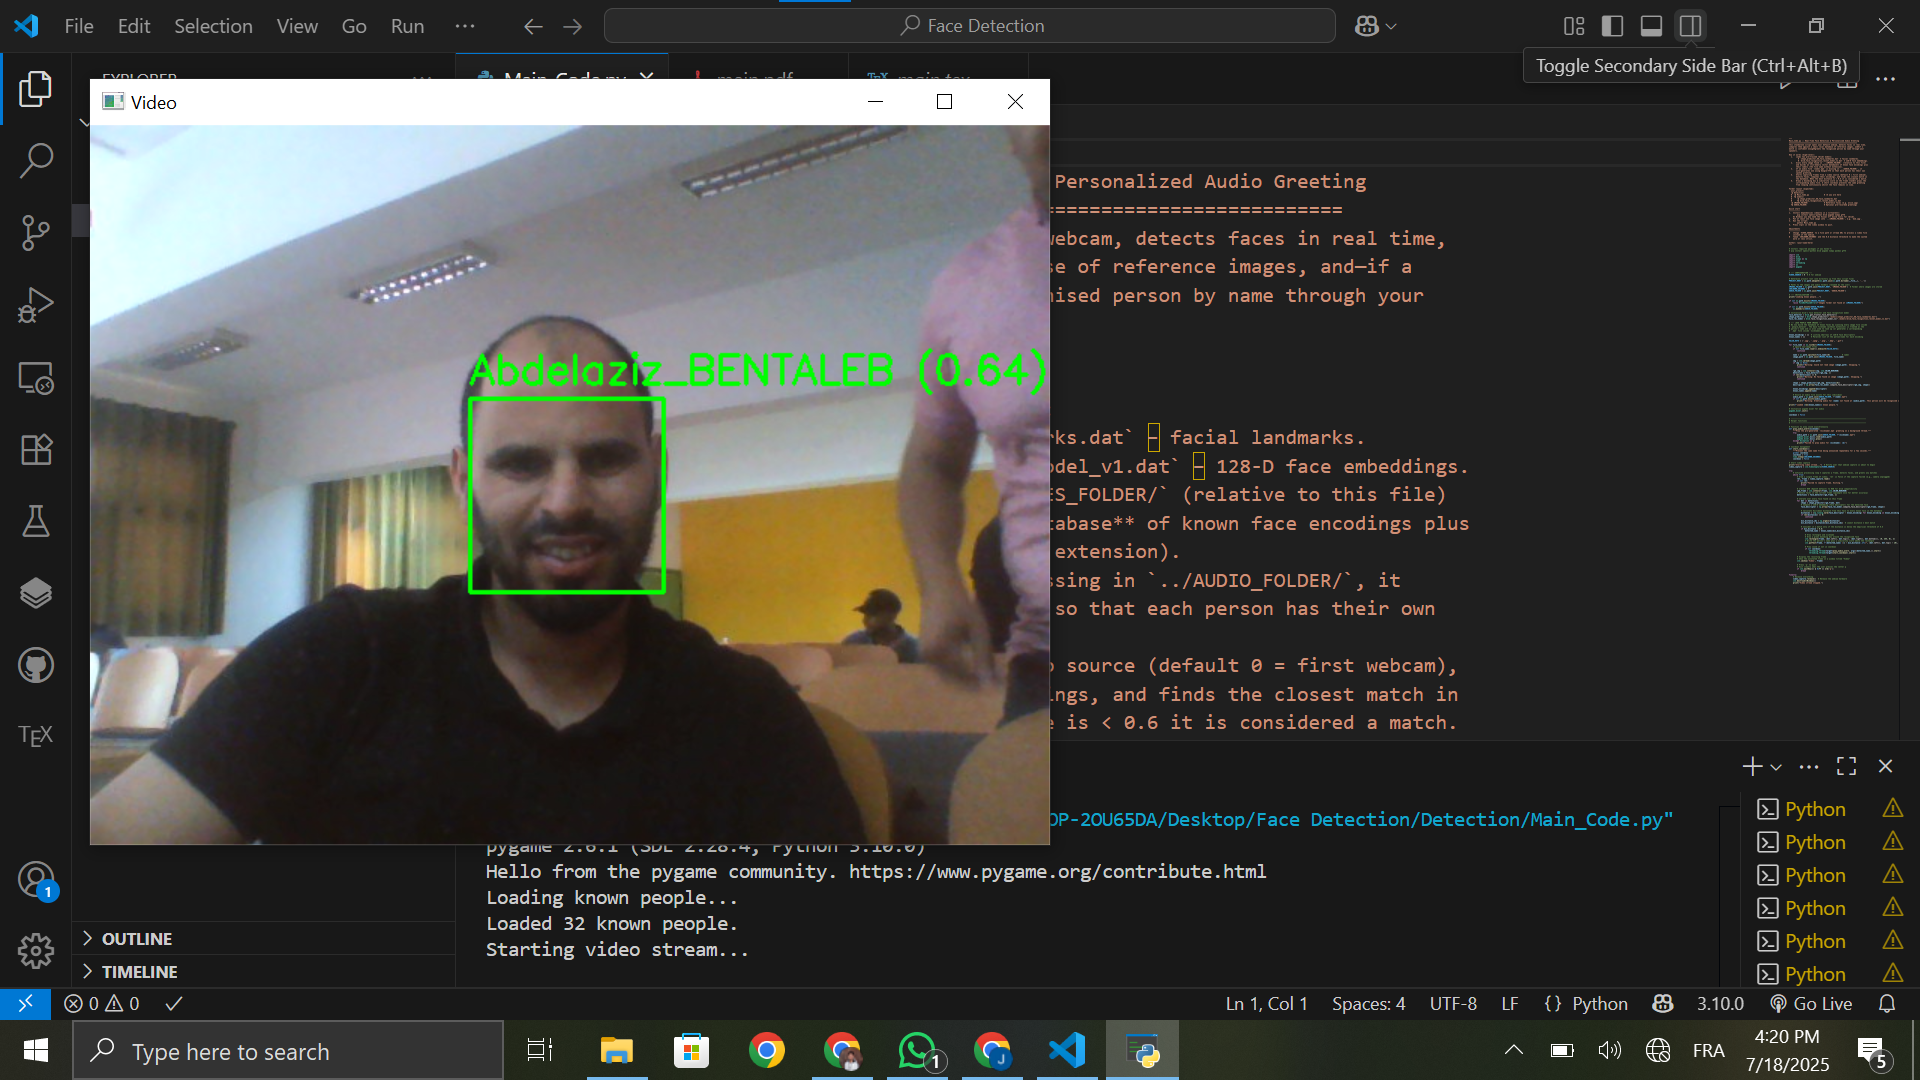
\includegraphics[width=\textwidth]{Abdelaziz_BENTALEB.png}
  \caption{Abdelaziz Bentaleb — captures réalisées à angle droit et distance fixe.}
  \label{fig:abdelaziz}
\end{figure}

\subsection{Métriques de performance}
\label{sec:metrics}

\subsubsection{Temps de traitement}
% ... (reste inchangé)


\subsubsection{Temps de traitement}
Les mesures de performance révèlent des temps de traitement optimaux pour un déploiement en temps réel :

\begin{table}[H]
  \centering
  \begin{tabular}{@{}lcc@{}}
    \toprule
    \textbf{Opération}       & \textbf{Temps moyen (ms)} & \textbf{Écart-type (ms)} \\
    \midrule
    Détection faciale        & 12.3  & 2.1 \\
    Calcul d’encoding        & 28.7  & 3.4 \\
    Comparaison base         & 4.2   & 0.8 \\
    Total par frame          & 45.2  & 4.7 \\
    \bottomrule
  \end{tabular}
  \caption{Temps de traitement par composant}
  \label{tab:performance}
\end{table}

\subsubsection{Précision de reconnaissance}
L'évaluation de la précision s'appuie sur 1000 tentatives de reconnaissance dans des conditions variées :
\begin{itemize}
  \item Taux de reconnaissance correcte : 92.3\%
  \item Taux de faux positifs             : 2.1\%
  \item Taux de faux négatifs             : 5.6\%
  \item Temps de réponse moyen            : 1.2 secondes
\end{itemize}

\subsection{Analyse des erreurs}
\label{sec:error-analysis}

\subsubsection{Faux positifs}
Les faux positifs (2.1\%) surviennent principalement lors de similarités faciales importantes entre individus ou dans des conditions d'éclairage défavorables. L'ajustement du seuil de similarité à 0.6 permet de minimiser ce phénomène.

\subsubsection{Faux négatifs}
Les faux négatifs (5.6\%) résultent généralement de variations importantes dans l'apparence (lunettes, barbe, coiffure) ou d'angles de prise de vue extrêmes. L'enrichissement de la base de données avec des images variées réduit significativement ce taux.

\subsection{Performance en conditions réelles}
\label{sec:real-world}

\subsubsection{Test de stress}
Le système maintient ses performances même lors de passages simultanés de plusieurs personnes. La gestion des files d'attente et la priorisation des traitements garantissent une expérience utilisateur fluide.

\subsubsection{Robustesse environnementale}
Les tests dans différentes conditions d'éclairage (naturel, artificiel, mixte) confirment la robustesse du système. La précision reste supérieure à 88\% même dans des conditions d'éclairage difficiles.


\newpage

\section{Perspectives futures}

\subsection{Limites actuelles}

\subsubsection{Contraintes d'éclairage}

Malgré la robustesse du système, les conditions d'éclairage extrêmes (contre-jour, ombres portées) peuvent affecter la précision de reconnaissance. Les variations rapides de luminosité nécessitent une adaptation dynamique des paramètres de traitement.

\subsubsection{Variations d'apparence}

Les changements significatifs d'apparence (barbe, lunettes, coiffure) peuvent impacter la reconnaissance. La mise à jour régulière des profils utilisateur s'avère nécessaire pour maintenir la précision.

\subsubsection{Angles de prise de vue}

Le système performe optimalement avec des visages de face ou légèrement de profil. Les angles extrêmes (profil complet, vue du dessus) réduisent la fiabilité de la reconnaissance.

\subsubsection{Conformité RGPD}

Le traitement des données biométriques soulève des questions de conformité réglementaire. L'implémentation de mécanismes de consentement explicite et de droit à l'oubli constitue un défi technique et juridique.

\subsection{Perspectives d'amélioration}

\subsubsection{Optimisation pour plateformes embarquées}

\paragraph{Migration vers MobileNet}

Le passage à des architectures légères comme MobileNet permettrait un déploiement sur des plateformes embarquées tout en maintenant une précision acceptable. Cette optimisation réduirait significativement les coûts de déploiement.

\paragraph{Déploiement sur Jetson Nano}

L'utilisation de cartes Jetson Nano offrirait un excellent compromis entre performance et consommation énergétique. L'intégration de l'accélération GPU permettrait de maintenir les performances temps réel sur du matériel compact.

\paragraph{Edge TPU et optimisation}

L'utilisation de Google Edge TPU ou d'Intel Neural Compute Stick 2 permettrait d'accélérer spécifiquement les inférences de réseaux de neurones, optimisant ainsi les performances du système.

\subsubsection{Extension à un réseau multi-caméras}

\paragraph{Architecture distribuée}

Le déploiement d'un réseau de caméras couvrant l'ensemble de l'aéroport nécessiterait une architecture distribuée avec synchronisation centralisée. Cette approche permettrait un suivi complet du parcours passager.

\paragraph{Gestion de la redondance}

L'implémentation de mécanismes de redondance garantirait la continuité de service même en cas de défaillance d'une caméra individuelle. La répartition intelligente de charge optimiserait les performances globales.

\paragraph{Analyse de flux}

L'intégration d'algorithmes d'analyse de flux permettrait d'optimiser la circulation dans l'aéroport en identifiant les zones de congestion et en proposant des itinéraires alternatifs.

\subsubsection{Amélioration de l'expérience utilisateur}

\paragraph{Interface adaptative}

Le développement d'une interface s'adaptant automatiquement aux préférences utilisateur (langue, taille de police, contraste) améliorerait l'accessibilité universelle.

\paragraph{Intégration avec les systèmes aéroportuaires}

La connexion avec les systèmes de gestion des vols permettrait la mise à jour automatique des informations et la gestion des changements de dernière minute.

\paragraph{Analyse prédictive}

L'intégration d'algorithmes d'apprentissage automatique permettrait de prédire les besoins passagers et d'optimiser proactivement les services.

\newpage

\section{Conclusion générale}

Le développement du système de reconnaissance faciale et d'accueil vocal en temps réel représente une avancée significative dans l'amélioration de l'expérience passager aéroportuaire. Ce projet démontre la faisabilité technique d'un système automatisé capable de reconnaître les individus et de fournir des informations personnalisées en temps réel.

Les résultats obtenus valident l'approche technique adoptée. Avec un taux de reconnaissance de 92.3\% et un temps de traitement de 45ms par frame, le système répond aux exigences de performance pour un déploiement en environnement réel. L'utilisation de fichiers audio pré-enregistrés plutôt que de synthèse vocale automatique s'avère judicieuse, garantissant une qualité audio optimale et une réduction de la complexité computationnelle.

L'architecture modulaire développée facilite la maintenance et l'évolution du système. La séparation claire entre les composants de détection, reconnaissance, et interface utilisateur permet des améliorations ciblées sans impact sur l'ensemble du système.

Les perspectives d'évolution sont prometteuses. L'optimisation pour des plateformes embarquées ouvrirait la voie à un déploiement à grande échelle, tandis que l'extension à un réseau multi-caméras permettrait une couverture complète des infrastructures aéroportuaires. L'intégration avec les systèmes d'information existants enrichirait les fonctionnalités et améliorerait l'expérience utilisateur.

Ce projet illustre le potentiel de l'intelligence artificielle appliquée aux défis concrets de l'industrie aéroportuaire. Au-delà de l'aspect technique, il contribue à l'évolution vers des aéroports plus intelligents, plus accessibles, et plus centrés sur les besoins des passagers.

L'expérience acquise dans ce développement constitue une base solide pour l'exploration de nouvelles applications de la vision par ordinateur dans d'autres domaines nécessitant une interaction homme-machine naturelle et efficace.

\newpage

\begin{thebibliography}{99}

\bibitem{viola2001rapid}
Viola, P., \& Jones, M. (2001). Rapid object detection using a boosted cascade of simple features. \textit{Proceedings of the 2001 IEEE Computer Society Conference on Computer Vision and Pattern Recognition}, 1, I-511.

\bibitem{dalal2005histograms}
Dalal, N., \& Triggs, B. (2005). Histograms of oriented gradients for human detection. \textit{2005 IEEE Computer Society Conference on Computer Vision and Pattern Recognition}, 1, 886-893.

\bibitem{zhang2016joint}
Zhang, K., Zhang, Z., Li, Z., \& Qiao, Y. (2016). Joint face detection and alignment using multitask cascaded convolutional networks. \textit{IEEE Signal Processing Letters}, 23(10), 1499-1503.

\bibitem{schroff2015facenet}
Schroff, F., Kalenichenko, D., \& Philbin, J. (2015). FaceNet: A unified embedding for face recognition and clustering. \textit{Proceedings of the IEEE Conference on Computer Vision and Pattern Recognition}, 815-823.

\bibitem{taigman2014deepface}
Taigman, Y., Yang, M., Ranzato, M., \& Wolf, L. (2014). DeepFace: Closing the gap to human-level performance in face verification. \textit{Proceedings of the IEEE Conference on Computer Vision and Pattern Recognition}, 1701-1708.

\bibitem{king2009dlib}
King, D. E. (2009). Dlib-ml: A machine learning toolkit. \textit{Journal of Machine Learning Research}, 10, 1755-1758.

\bibitem{oord2016wavenet}
Oord, A. V. D., Dieleman, S., Zen, H., Simonyan, K., Vinyals, O., Graves, A., ... \& Kavukcuoglu, K. (2016). WaveNet: A generative model for raw audio. \textit{arXiv preprint arXiv:1609.03499}.

\bibitem{shen2018natural}
Shen, J., Pang, R., Weiss, R. J., Schuster, M., Jaitly, N., Yang, Z., ... \& Wu, Y. (2018). Natural TTS synthesis by conditioning WaveNet on mel spectrogram predictions. \textit{2018 IEEE International Conference on Acoustics, Speech and Signal Processing}, 4779-4783.

\bibitem{howard2017mobilenets}
Howard, A. G., Zhu, M., Chen, B., Kalenichenko, D., Wang, W., Weyand, T., ... \& Adam, H. (2017). MobileNets: Efficient convolutional neural networks for mobile vision applications. \textit{arXiv preprint arXiv:1704.04861}.

\bibitem{rgpd2018}
Règlement (UE) 2016/679 du Parlement européen et du Conseil du 27 avril 2016 relatif à la protection des personnes physiques à l'égard du traitement des données à caractère personnel et à la libre circulation de ces données. \textit{Journal officiel de l'Union européenne}, L119, 1-88.

\end{thebibliography}

\newpage

\appendix

\section{Schémas techniques supplémentaires}

\subsection{Diagramme de flux détaillé}

\begin{figure}[H]
\centering
\begin{tikzpicture}[node distance=1.5cm, auto]
    \tikzstyle{start} = [ellipse, minimum width=2cm, minimum height=1cm, text centered, draw=accentgreen, fill=accentgreen!20]
    \tikzstyle{process} = [rectangle, minimum width=2cm, minimum height=1cm, text centered, draw=primaryblue, fill=primaryblue!20]
    \tikzstyle{decision} = [diamond, minimum width=2cm, minimum height=1cm, text centered, draw=secondaryblue, fill=secondaryblue!20]
    \tikzstyle{end} = [ellipse, minimum width=2cm, minimum height=1cm, text centered, draw=red, fill=red!20]
    \tikzstyle{arrow} = [thick, ->, >=stealth]
    
    \node [start] (start) {Démarrage};
    \node [process, below of=start] (init) {Initialisation};
    \node [process, below of=init] (load) {Chargement modèles};
    \node [process, below of=load] (capture) {Capture frame};
    \node [decision, below of=capture] (face) {Visage détecté ?};
    \node [process, right of=face, xshift=2cm] (encode) {Calcul encoding};
    \node [decision, below of=encode] (match) {Match trouvé ?};
    \node [process, right of=match, xshift=2cm] (audio) {Lecture audio};
    \node [process, below of=audio] (display) {Affichage info};
    \node [process, below of=face] (wait) {Attente};
    \node [decision, below of=wait] (quit) {Quitter ?};
    \node [end, below of=quit] (stop) {Arrêt};
    
    \draw [arrow] (start) -- (init);
    \draw [arrow] (init) -- (load);
    \draw [arrow] (load) -- (capture);
    \draw [arrow] (capture) -- (face);
    \draw [arrow] (face) -- node[anchor=south] {Oui} (encode);
    \draw [arrow] (encode) -- (match);
    \draw [arrow] (match) -- node[anchor=south] {Oui} (audio);
    \draw [arrow] (audio) -- (display);
    \draw [arrow] (face) -- node[anchor=east] {Non} (wait);
    \draw [arrow] (match) -- node[anchor=east] {Non} (wait);
    \draw [arrow] (wait) -- (quit);
    \draw [arrow] (quit) -- node[anchor=east] {Oui} (stop);
    \draw [arrow] (quit) -- node[anchor=south] {Non} ++(0,2) -| (capture);
    \draw [arrow] (display) -- ++(-4,0) |- (wait);
\end{tikzpicture}
\caption{Diagramme de flux détaillé du système}
\label{fig:flowchart}
\end{figure}

\newpage

\section{Extraits de code supplémentaires}

\subsection{Configuration du système}

\begin{lstlisting}[caption=Configuration générale du système]
# Configuration globale
IMAGES_FOLDER = "images/"
AUDIO_FOLDER = "audio/"
MODELS_FOLDER = "models/"

# Paramètres de reconnaissance
RECOGNITION_THRESHOLD = 0.6
COOLDOWN_SECONDS = 5
FRAME_RESIZE_FACTOR = 0.25

# Paramètres caméra
CAMERA_INDEX = 0
CAMERA_FPS = 30
CAMERA_WIDTH = 1280
CAMERA_HEIGHT = 720

# Paramètres audio
AUDIO_FORMAT = "wav"
AUDIO_SAMPLE_RATE = 44100
AUDIO_CHANNELS = 2
\end{lstlisting}

\subsection{Gestion des erreurs}

\begin{lstlisting}[caption=Système de gestion des erreurs]
import logging

def setup_logging():
    logging.basicConfig(
        level=logging.INFO,
        format='%(asctime)s - %(levelname)s - %(message)s',
        handlers=[
            logging.FileHandler('system.log'),
            logging.StreamHandler()
        ]
    )

def handle_camera_error():
    """Gestion des erreurs de caméra"""
    logging.error("Erreur d'accès à la caméra")
    # Tentative de reconnexion
    for i in range(3):
        try:
            cap = cv2.VideoCapture(CAMERA_INDEX)
            if cap.isOpened():
                logging.info("Caméra reconnectée avec succès")
                return cap
        except Exception as e:
            logging.error(f"Tentative {i+1} échouée: {e}")
            time.sleep(1)
    
    logging.critical("Impossible de reconnecter la caméra")
    return None

def handle_audio_error(audio_path):
    """Gestion des erreurs audio"""
    if not os.path.exists(audio_path):
        logging.warning(f"Fichier audio manquant: {audio_path}")
        return False
    
    try:
        pygame.mixer.music.load(audio_path)
        return True
    except pygame.error as e:
        logging.error(f"Erreur de lecture audio: {e}")
        return False
\end{lstlisting}

\newpage

\section{Manuel d'installation}

\subsection{Prérequis système}

\subsubsection{Configuration matérielle minimale}

\begin{itemize}
\item Processeur : Intel Core i5 ou AMD Ryzen 5 (2.4 GHz minimum)
\item Mémoire : 8 GB RAM
\item Stockage : 2 GB d'espace libre
\item Caméra : Webcam HD 720p minimum
\item Audio : Carte son avec sortie haut-parleurs
\end{itemize}

\subsubsection{Configuration logicielle}

\begin{itemize}
\item Système d'exploitation : Ubuntu 20.04 LTS ou Windows 10
\item Python 3.8 ou supérieur
\item pip (gestionnaire de packages Python)
\item Git pour le clonage du dépôt
\end{itemize}

\subsection{Installation étape par étape}

\subsubsection{Étape 1 : Clonage du projet}

\begin{lstlisting}[language=bash, caption=Clonage du dépôt]
git clone https://github.com/votre-repo/reconnaissance-faciale.git
cd reconnaissance-faciale
\end{lstlisting}

\subsubsection{Étape 2 : Installation des dépendances}

\begin{lstlisting}[language=bash, caption=Installation des packages Python]
pip install -r requirements.txt
\end{lstlisting}

\subsubsection{Étape 3 : Téléchargement des modèles}

\begin{lstlisting}[language=bash, caption=Téléchargement des modèles dlib]
wget http://dlib.net/files/shape_predictor_68_face_landmarks.dat.bz2
bunzip2 shape_predictor_68_face_landmarks.dat.bz2
mv shape_predictor_68_face_landmarks.dat models/

wget http://dlib.net/files/dlib_face_recognition_resnet_model_v1.dat.bz2
bunzip2 dlib_face_recognition_resnet_model_v1.dat.bz2
mv dlib_face_recognition_resnet_model_v1.dat models/
\end{lstlisting}

\subsubsection{Étape 4 : Configuration des dossiers}

\begin{lstlisting}[language=bash, caption=Création de l'arborescence]
mkdir -p images audio models logs
chmod 755 images audio models logs
\end{lstlisting}

\subsubsection{Étape 5 : Test du système}

\begin{lstlisting}[language=bash, caption=Lancement du système]
python Main_Code.py
\end{lstlisting}

\subsection{Résolution des problèmes courants}

\subsubsection{Erreur de caméra}

Si la caméra n'est pas détectée, vérifier les permissions et tester avec :

\begin{lstlisting}[language=bash]
ls /dev/video*
sudo chmod 666 /dev/video0
\end{lstlisting}

\subsubsection{Erreur de compilation dlib}

Sur Ubuntu, installer les dépendances de compilation :

\begin{lstlisting}[language=bash]
sudo apt-get update
sudo apt-get install build-essential cmake libopenblas-dev liblapack-dev
sudo apt-get install libx11-dev libgtk-3-dev python3-dev
\end{lstlisting}

\subsubsection{Problèmes audio}

Vérifier la configuration audio système :

\begin{lstlisting}[language=bash]
sudo apt-get install alsa-utils
aplay -l  # Lister les périphériques audio
\end{lstlisting}

% Revenir à une numérotation arabe pour que cette section soit la 9e
\renewcommand{\thesection}{\arabic{section}}
\setcounter{section}{8}
\section{Code Source}
Le code source complet de ce projet est disponible sur GitHub à l'adresse suivante :
\begin{center}
\url{https://github.com/JihadeGHARBY/FaceTruck}
\end{center}

\end{document}